\section{Le POSIX 1003.1}
 
Traditionnellement les systèmes qui implémentaient la norme POSIX avaient un système simple et puissant de permissions mais qui cependant posait certains problèmes. En effet, les différentes versions d'ACL disponibles étaient incompatibles entre elles.
 
Pour normaliser les problème de sécurité sur les systèmes POSIX (ACL en faisant partie), un groupe a été formé pendant la définition de la famille de normes POSIX 1003.1. Les premiers documents POSIX qui ont pris en compte ces questions étaient les documents 1003.1e (\emph{System Application Programming Interface}) et 1003.2c (\emph{Shell and Utilities}), cependant, le premier draft était trop ambitieux. En effet, le groupe responsable pour la normalisation avait divisé ses efforts sur un grand nombre de domaines qui comportaient les \emph{Access Control Lists} (ACL), les \emph{Audit}, les \emph{Capability},les \emph{ Mandatory Access Control }(MAC), et l'\emph{Information Labeling}\cite{aclsuse}.
 
En Janvier de 1998\cite{aclsuse} le financement pour ce projet à été suspendu, par contre, le travail n'était pas prêt. De toute façon le dixsèptieme draft a quand même été rendu public\cite{posix17}.
 
Après cette publication, des systèmes UNIX appelés "\emph{trusted}" (Trusted Solaris, Trusted Irix, Trusted AIX) ont été développés à partir du draft 17. Ces systèmes ne sont pas complètement compatibles entre eux. Heureusement aujourd'hui la plupart des systèmes UNIX et UNIX-like supportent les ACL. Ces implémentations sont usuellement compatibles avec le draft 17. Le projet TrustedBSD implémente aussi les ACL sur les système BSD. Les ACL sont apparues sur les Macs en 2003 avec la RELEASE MAC FreeBSD.
 
Les ACL sont une évolution du système de permissions traditionnel présent dans pratiquement tous les systèmes UNIX, alors, avant d'expliquer les ACL on va d'abord parler du modèle traditionnel.
 
\subsection*{Système de permissions traditionnel}
 
%Les groups et les permissions
Le modèle traditionnel POSIX offre trois classes d'utilisateurs qui sont: le propriétaire (\emph{owner}), le groupe propriétaire (\emph{group}) et les autres utilisateurs (\emph{others}). Chaque groupe a un octet que indique les permissions de lecture (\emph{\textbf{r}ead}), d'écriture (\emph{\textbf{w}rite}) et d'exécution (\emph{e\textbf{x}ecute}).
 
%Explication simple
Après les trois octets peut venir le \emph{Set User Id}, \emph{Set Group Id} et le \emph{Sticky Bit} qui peuvent être utilisés dans certain cas. Il faut faire attention avec le \emph{Sticky Bit}, il permet aux utilisateurs normaux d'exécuter les utilitaires comme l'administrateur(\emph{root}), donc une faille de sécurité dans une application utilisant le \emph{Sticky Bit} peut compromettre le système entier.
 
%Le droit du root
Seul le \emph{root} peut créer les groupes et changer les associations de groupes. Il peut aussi changer les propriétaires.
 
\subsection*{Les ACL}
 
%Definitions de base
Chaque ACL est une ensemble de règles d'accès. Dans une modèle de sécurité utilisant les ACL, si une entité fait une requête pour accéder aux données, il faut consulter les la liste d'ACL pour savoir si nous avons la permission pour l'opération demandé. Les règles possibles peuvent être consultées dans le tableau ci-dessous(\ref{entree}).

\begin{center}
\begin{tabular}{|l|l|}
  \hline
    \multicolumn{2}{|c|}{Les types de ACL} \\
  \hline
\textbf{Type d'entrée} & \textbf{format} \\
  \hline
Propriétaire & user::rwx \\
Utilisateur nommée & user:name:rwx \\
Groupe propriétaire & group::rwx \\
Groupe nommée & group:name:rwx \\
Masque & mask::rwx \\
Autres & other::rwx \\
  \hline
\end{tabular}
\label{tab:entree}
\end{center}
 
Les règles sont formées par un indicateur de classe (comme les classes du système traditionnel), l'identificateur pour préciser de quel utilisateur ou groupe on parle puis les octets de permissions.
 
%REFAIRE -----------------------------------------------------------------------------------
Avec cette représentation le sens de la classe du groupe a été redéfini comme le limite supérieur de les permission de chaque entrée dans la classe du groupe. C'était a dire que les entrée du groupe et du utilisateur nommées seront désigner à entrée du groupe. Aussi, c'est importante rappeler que cette choix permettre se prémunir contre les application qui ne sont pas conscient de les ACL.
\footnote{Fabricio: Je ne comprend pas bien cette affirmation, je laisse ici le teste orignial:
These named group and named user entries are assigned to the group class, which already contains the owning group entry. Different from the POSIX.1 permission model, the group class may now contain ACL entries with different permission sets, so the group class permissions alone are no longer sufficient to represent all the detailed permissions of all ACL entries it contains. Therefore, the meaning of the group class permissions is redefined: under their new semantics, they represent an upper bound of the permissions that any entry in the group class will grant. This upper bound property ensures that POSIX.1 applications that are unaware of ACLs will not suddenly and unexpectedly start to grant additional permissions once ACLs are supported.}.
 
Les ACL équivalentes au mode simple de permissions s'appellent les ACL minimales. Si les ACL possèdent des entrées supplémentaires, ont les appelle ACL étendues. Toutes les ACL étendues doivent avoir une entrée masque et peuvent contenir théoriquement autant d'entrées que l'on désire. On verra après que ce numéro d'entrée peut-être limitée pour chaque implémentation et qu'il est aussi important pour les performances.
 
%EXPLIQUER MIEUX
Dans les ACL étendues on peut avoir des entrées avec plusieurs utilisateurs et/ou groupes, quelques de cette entrées peut-être contenir permissions qui la classe groupe n'aurais pas, alors, on peut avoir une inconsistance basée en le cas qui les permissions du groupe propriétaire sont diffèrent de les permission de la classe groupe.

%%%%%%%%%%%%%%%%%%%%%%%%%%%%%%%%%%%%%%%%%%%%%%%%%%%%%%%%%%%%%%%%%%%%%%%%%%%%%%%%%%%%%%%%%%%%%%
 
On peut résoudre ce problème avec un masque. Comme on peut l'observer dans le figure (\ref{fig:img_acl-mapping}), il y a deux cas:  Les ACL minimales où la classe groupe est référencée pour l'entrée du groupe propriétaire. Les ACL étendues de la classe groupe seront trouvées en faisant un masque avec les permissions du groupe propriétaire et les permissions des utilisateurs nommés mais si l'entrée de permission du groupe propriétaire possède des droits supérieurs au masque ils seront conservés. Cela rend difficile le calcul de classe groupe. 

\begin{figure}[htbp]
\centering
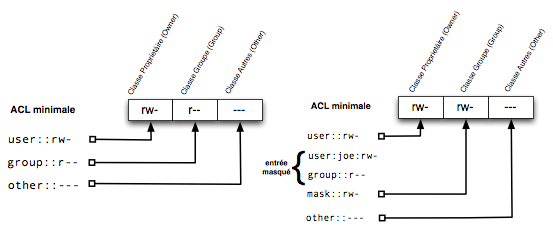
\includegraphics[height=3in]{img/acl-mapping.jpg}
\caption{caption}
\label{fig:img_acl-mapping}
\end{figure}
 
 
Pour assurer le consistance/cohérance, quand une application change les permissions (par exemple le commande \emph{chmod}) les ACL sont modifiée de façon a reproduire cette modification.
 
On a dit que le permission de la classe groupe est calculée comme la limite supérieur de tous les entrée dans le classe group. Avec les ACLs minimaux cette computation est simple, par contre, avec les ACLs étendu, on a besoin de masquer les permissions. Comme l'exemple de le tableau (\ref{tab:masquee}), les entrée de permission qui sont partie de la classe de groupe et qui aussi sont présente dans l'entrée masque sont applique effectivement. Si une permission était absent dans le masque, c'est a dire que aucun entrée de group (qui non le groupe du propriétaire) peut avoir ce permission, on dit dans ce cas qui la entrée est masquée.
 
\begin{center}
\begin{tabular}{|l|l|l|}
  \hline
    \multicolumn{3}{|c|}{La masque de permissionL} \\
  \hline
\textbf{Type} & \textbf{Format} & \textbf{Permission} \\
  \hline
Utilisateur nommée & user:jean:r-x & r-x\\
  \hline
Masque & mask::rw- & rw-\\
  \hline
\multicolumn{2}{|c|}{Permission Effective} & r--\\
  \hline
\end{tabular}
\label{tab:masque}
\end{center}
 
\subsection*{Algorithme de vérification}
 
Pour vérifier les droits d'accès d'une objet du système de fichier, il y a une algorithme assez simple.\footnote{Il faut traduire cette algorithme lá :-)}
 
%changer le titre et la langue
\begin{algorithm}
\caption{Vérifie se une utilisateur peut ou ne peut pas accéder une objet du système de fichier}
\label{algacl}
\begin{algorithmic}
\IF{the user ID of the process is the owner}
\STATE the owner entry determines access
\ELSIF{the user ID of the process matches the qualifier in one of the named user entries}
\STATE this entry determines access
\ELSIF{one of the group IDs of the process matches the owning group and the owning group entry contains the requested permissions}
\STATE this entry determines access
\ELSIF{one of the group IDs of the process matches the qualifier of one of the named group entries and this entry contains the requested permissions}
\STATE this entry determines access
 
\ELSIF{one of the group IDs of the process matches the owning group or any of the named group entries, but neither the owning group entry nor any of the matching named group entries contains the requested permissions}
\STATE this determines that access is denied
 
\ELSE
\STATE the other entry determines access.
\ENDIF
 
 
\IF{the matching entry resulting from this selection is the owner or other entry and it contains the requested permissions}
\STATE access is granted
\ELSIF{the matching entry is a named user, owning group, or named group entry and this entry contains the requested permissions and the mask entry also contains the requested permissions (or there is no mask entry)}
\STATE access is granted
 
\ELSE
\STATE access is denied.
\ENDIF
\end{algorithmic}
\end{algorithm}
 
 
\subsection*{Héritage mécanisme}
 
Le système POSIX règle non seulement les accès aux objets du système, mais aussi sur le mécanisme d'Héritage. Les ACL sont partagés en deux types, les \emph{access ACL} (qu'on a vu jusqu'á maintenant) et les \emph{default ACL} qui comprennent les règles d'héritage.
 
Quand on parle de l'héritage, on parle des droits qui sont attribue aux objet du système pendant au moment où ils sont crées. Il y un seul type d'objet qui peut être associe avec les \emph{default ACL}; les répertoire. Il faut dire que il n'y a aucune sens en donne \emph{default ACL } pour les fichiers, alors que, aucune objet du système peut être crée dans une fichier, aussi, il faut rappeler que les \emph{Default ACL} n'ont pas aucune implication sur les \emph{access ACL}.
 
Si un répertoire est crée dans une autre, si le première répertoire a \emph{default ACL}, d'accord avec le mécanisme de héritage, le deuxième aurais le même ACL qui le première (\emph{default} et \emph{access}). Les objets qui ne sont pas répertoire, devons hérite les \emph{access ACL} seulement.
 
Chaque \emph{system call} que crée les objets du système de fichier a une \emph{mode parameter}. Ce paramètre peut contenir neuve octet de permission pour chaque classe (propriétaire, groupe et les autres). Les permission effective de chaque objet crée est l'intersection de les permission défini pour les \emph{default ACL} et les spécification dans le \emph{mode parameter}.
 
Le système traditionnel a une commande pour designer les modes de permission par défaut pour les nouveau fichiers et répertoires: le commande \emph{umask}. Quand il n'y a aucune \emph{default ACL}, le permission effective est détermine par le paramètre de mode moins les permission configuré avec \emph{umask}.
 
